\chapter{Lecture 21}
Regarding our discussion of interpolation from the previous lecture, what if instead of observing our ground truth function $f$, we instead observe $f + \eta$ with noise $\eta$? 
\section{Cross-validation}
Cross-validation is a class of techniques used to assess the generalizability of a model to different data sets. The central idea behind cross-validation is to interpolate a target function $f$ on a proper subset of its domain and then check the error on all the data points that were not considered during the initial interpolation. If this error is low, we may be more confident in our interpolation's generalizability.

\subsection{Linear regression with leave-$p$-out cross-validation}
We motivate this process with an example with linear regression. We are given observations $Y=\{\bs{y}_1,...,\bs{y}_J\} \subseteq \R^{d}$ with
\begin{align}
    \bs{y}_j = \bs{f}_j + \bs{\eta}_j
\end{align}
and $\bs{f}_j \approx \bs{f}(\bs{x}_j)$ for target $\bs{f}$ and noise $\bs{\eta}_j$. In linear regression, we wish to solve for $\bs{\alpha}$ and $\bs{\beta}$ such that
\begin{ceqn} \label{eqn:21:linreg}
    L = \sum_{j=1}^{J} \left(\bs{y}_j - \hat{\bs{y}}_j\right)^2 \\
    \hat{\bs{y}}_{j} = \bs{\alpha} + \bs{\beta} \cdot \bs{x}_j
\end{ceqn}
is minimized. Our approach in this example will be \bt{leave-$p$-out} cross-validation. We first select a valid set $V = \{\bs{y}_{j_1},...,\bs{y}_{j_p}\}$ and a training set $T = Y \setminus V$. We then solve the auxiliary problem to find $\bs{\alpha}_{0}$ and $\bs{\beta}_{0}$ such that
\begin{align} \label{eqn:21:linregaux}
L_{T} &:= \sum_{j \in T} \left( \bs{y}_{j} - \hat{\bs{y}}_{j} \right)^2 
\end{align}
is minimized. The validation error is then defined by
\begin{ceqn} \label{eqn:21:linregval}
    L_{V} &:= \sum_{j \in V} \left( \bs{y}_j - \hat{\bs{y}_{j,T}} \right)^2 \\
    \hat{\bs{y}}_{j,T} &:= \bs{\alpha}_0 + \bs{\beta}_0 \cdot \bs{x}_{j}.
\end{ceqn}
Finally, we define the total cross-validation error as
\begin{align} \label{eqn:21:crossval}
    L_{cross} := \sum_{V \in \mathcal{V}} L_{V}
\end{align}
where
\begin{align} \label{eqn:21:v}
\mathcal{V} := \{ V \subseteq Y : |V|=p \}.
\end{align}
Note that Equations \eqref{eqn:21:crossval} and \eqref{eqn:21:v} express that we exhaustively check validation sets of size $p$. This may be untenable for large $J$ and $p$ since 
\begin{align*}
    |\mathcal{V}| = \binom{J}{p}
\end{align*}
grows very quickly with $J$ as long as $p$ is reasonably far away from $0$ and from $J$.
In the case of linear regression, it can be shown that the expected cross-validation loss is given by
\begin{align} \label{eqn:21:lossest}
\EE{L} = \frac{n-p-1}{n+p+1} \EE{L_{cross}}.
\end{align}
Equation \eqref{eqn:21:lossest} can be used to determine whether we are overfitting our data when using linear regression. A figure showing this phenomenon can be seen below.
\begin{figure}
    \centering
    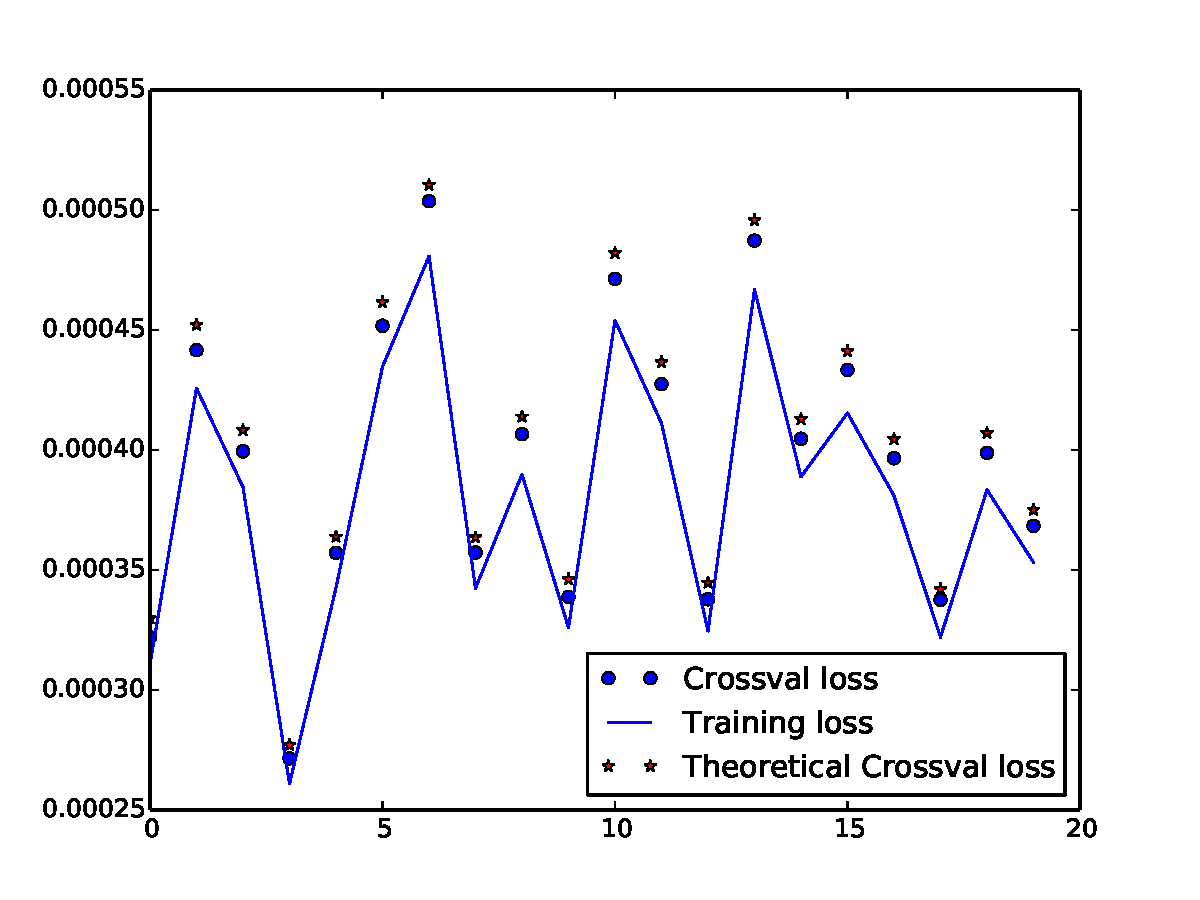
\includegraphics[width=\textwidth]{images/linreg-crossval.pdf}
    \caption{Code to produce this figure can be found \href{https://github.com/tmasthay/MathModeling/tree/main/lectures/lecture21}{here}.}
    \label{fig:21:crossval}
\end{figure}

\section{Choice of norms}
Say we have observations $\bs{f} = (f(\bs{x}_1),...,f(\bs{x}_n))^{T}$. Note that the optimization outlined in Equation \eqref{eqn:21:linregaux} is possibly the most common for approximation, i.e., least-squares or $L^2$ minimization.
However, we do not need to minimize with respect to $L^2$ for approximation, and in some contexts, we may be better off using a different norm. 

In general, $L^2$ is (a) a compromise between $L^{\infty}$ and $L^{1}$ minimization, (b) has ``good statistical properties'' in some sense, and (c) lends itself to efficient numerical algorithms. $L^1$ minimization is typically more robust than $L^2$ with respect to noise. Intuitively, this is because the squaring of the difference exacerbates the effect of an outlier. Finally, $L^{\infty}$ is very sensitive to noise because it exacerbates this outlier issue even more than $L^2$. $L^{\infty}$ typically finds its application for softwares such as numerical libraries for worst-case bounds on the error of approximations for evaluations such as Taylor series. \askbjorn{Draw informative pictures to outline here}. There are obviously many other norms to optimize with, but this is beyond the scope of our discussion.

As far as computational methods, $L^2$ optimization is usually solved with the normal equations. These can be solved without matrix decomposition or with the QR decomposition or SVD. These decompositions are more robust but more expensive. $L^1,L^{\infty}$ optimization are typically solved through linear programming. The general form for linear programming is given below.
\begin{ceqn}
    &\min_{\bs{x} \in \mathbb{R}^{n}} \bs{c} \cdot \bs{x} \\
    &\textup{subject to } \bs{A} \bs{x} - \bs{b} \leq \bs{0}, \bs{x} \geq \bs{0} 
\end{ceqn}